%ब 
\section{Delete} \label{s:results-Delete}

A \texttt{delete} operation triggers a referential integrity validation whenever
any entity is deleted in the experiments.
Figure~\ref{fres:Delete} presents the results of a single \texttt{delete} on
each entity for all the solutions.
Figure~\ref{fres:Delete-responsetime} shows the time taken to perform a single
\texttt{delete} on each entity in the solutions and
Figure~\ref{fres:Delete-throughput} presents the throughput for this operation.

	\begin{figure}[H] 
	\newcommand{\W}{.5\textwidth}
		\subfigure[Response time for Update operation]
		{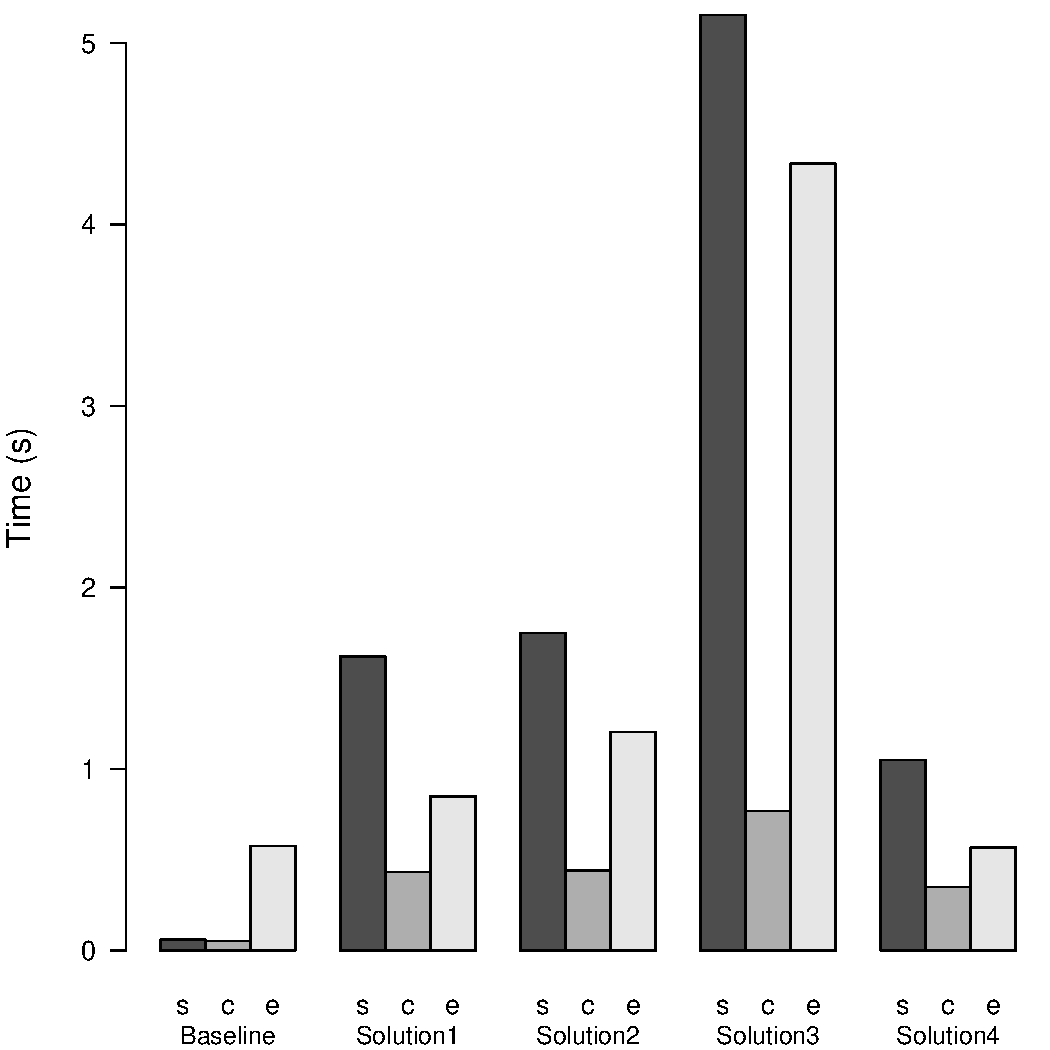
\includegraphics[width=\W]{figure/result/barplot-delete-rt.pdf}\label{fres:Delete-responsetime}}
		\subfigure[Throughput for Update operation]
		{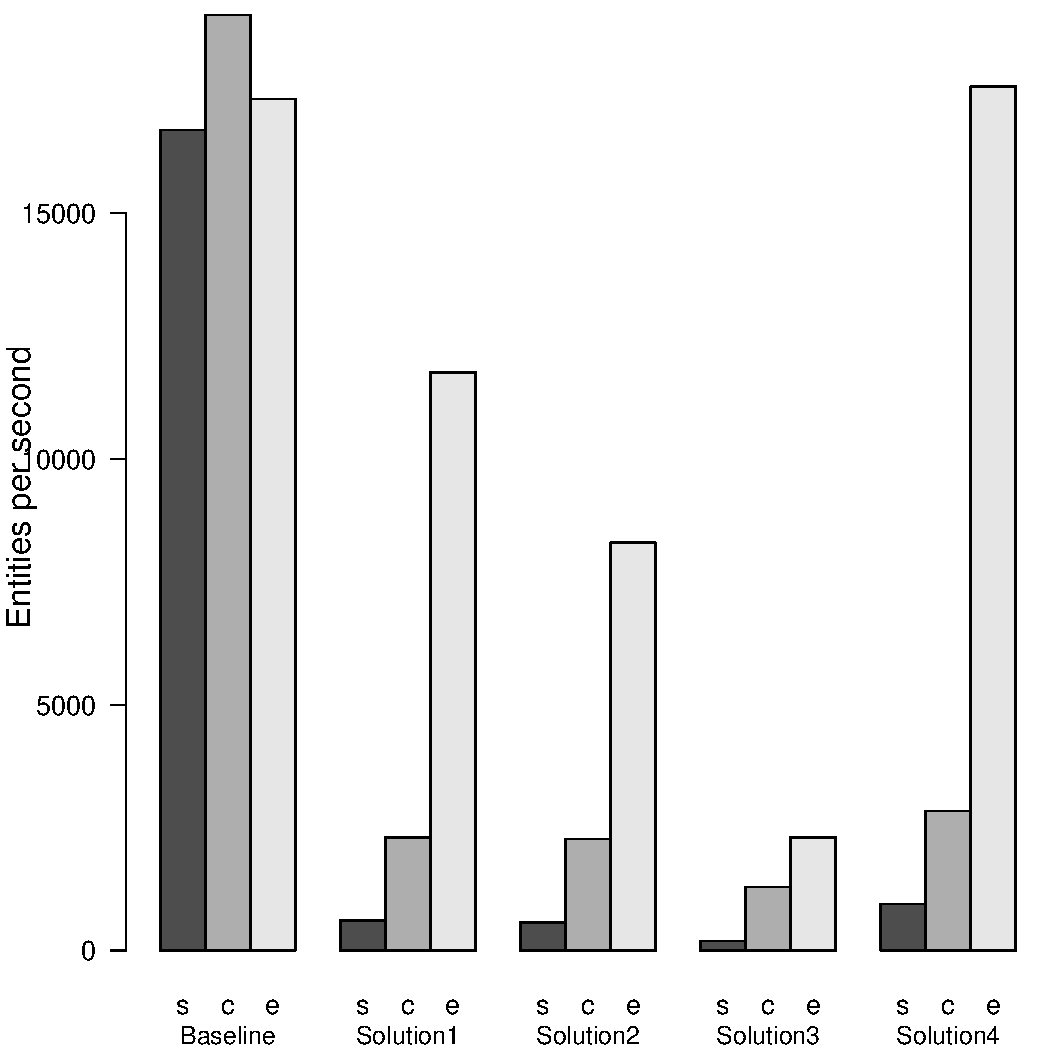
\includegraphics[width=\W]{figure/result/barplot-delete-tp.pdf}\label{fres:Delete-throughput}}
		\caption{Performance of Solutions in Update}\label{fres:Delete}
	\end{figure}
 
It can be seen from the results that the \texttt{delete} on \texttt{Enrolment}
is the fastest in all the solutions, while  \texttt{delete} on a
\texttt{Student} entity takes the most time. \texttt{delete} on a
\texttt{Course} entity always takes more time than \texttt{delete} on
\texttt{Enrolment} but is faster than deleting \texttt{Student} entities.

As seen in \texttt{update}, the difference in the performance of the operation
on the different entities are because of the referential integrity rules on
child and parent entities. Deleting \texttt{Enrolment} entities do not invoke
any referential integrity validations since it has no child dependencies on it.
However, this operation is  slower than the baseline in all the solutions
because it involves accessing metadata to retrieve its relevant constraints in
order to determine if it has any child dependencies or not.

Deleting \texttt{Student} entities is a cascaded operation which involves
deleting the child dependencies in the \texttt{Enrolment} column family.
Accessing the relevant constraints and  \texttt{Enrolment} to delete the child
entities that have a reference to the \texttt{Student} causes \texttt{delete} to
consume more time to complete. Similarly, \texttt{delete} on \texttt{Course}
entities also involves accessing the relevant constraints and finding the child
dependencies in \texttt{Enrolment}. However, in the experiments  all the
entities in \texttt{Enrolment} is deleted before \texttt{delete} is invoked on
\texttt{Course} entities. This allows the \texttt{Course} entities to be deleted
despite having a \texttt{NoDelete} \texttt{DeleteRule}. Thus, \texttt{delete} on
\texttt{Course} involves the time to access metadata and to search for any
existing child dependencies in \texttt{enrolment} and values are deleted from a
single column family. Note that \texttt{delete} on \texttt{Student} entities
involve deleting values from two column families.


The Figures~\ref{fres:delete-user},~\ref{fres:delete-course}
and~\ref{fres:delete-enrolment} show the response time and throughput of a
\texttt{delete} operation on the different entities in the solutions.
Figure~\ref{fres:delete-user} presents the results for a \texttt{delete} on a
\texttt{student} entity and Figures~~\ref{fres:delete-course}
and~\ref{fres:delete-enrolment} show the results for a \texttt{delete} on a
\texttt{Course} and \texttt{Enrolment} entity. It can be seen from these results
that Solution~4 takes the least time to complete a \texttt{delete} operation on
each entity, while Solution~3 takes the most time. Solution~4 caches the
metadata of all the entities and avoids multiple accesses to the
\texttt{Metadata} column family but Solution~3 requires accessing
\texttt{Metadata} each time a constraint has to be accessed for an entity. The
performance of Solutions~1 and 2 are comparable to each other even though
Solution~2 takes slightly more time due to its additional search operation to
locate the top row.

When compared to the baseline, all the solutions take longer to delete entities.
As mentioned previously, this is because all the solutions involve accessing
relevant constraints and performing validations. Solution~4 is almost similar
the baseline when \texttt{Enrolment} and \texttt{Course} entities are deleted,
which shows that accessing the metadata does not cause much difference in the
performance. Solutions~1 and 2 are almost twice slower than baseline in such
cases. However, in a cascaded delete which includes referential integrity
validations it is almost 17 times slower than the baseline whereas Solution~3 is
almost 80 times slower. In this case, Solutions~1 and 2 are only slightly slower
than the baseline.



\newpage
		\begin{figure}[H]
		\centering
		\newcommand{\W}{.4\textwidth}
			\subfigure[Response time]
			{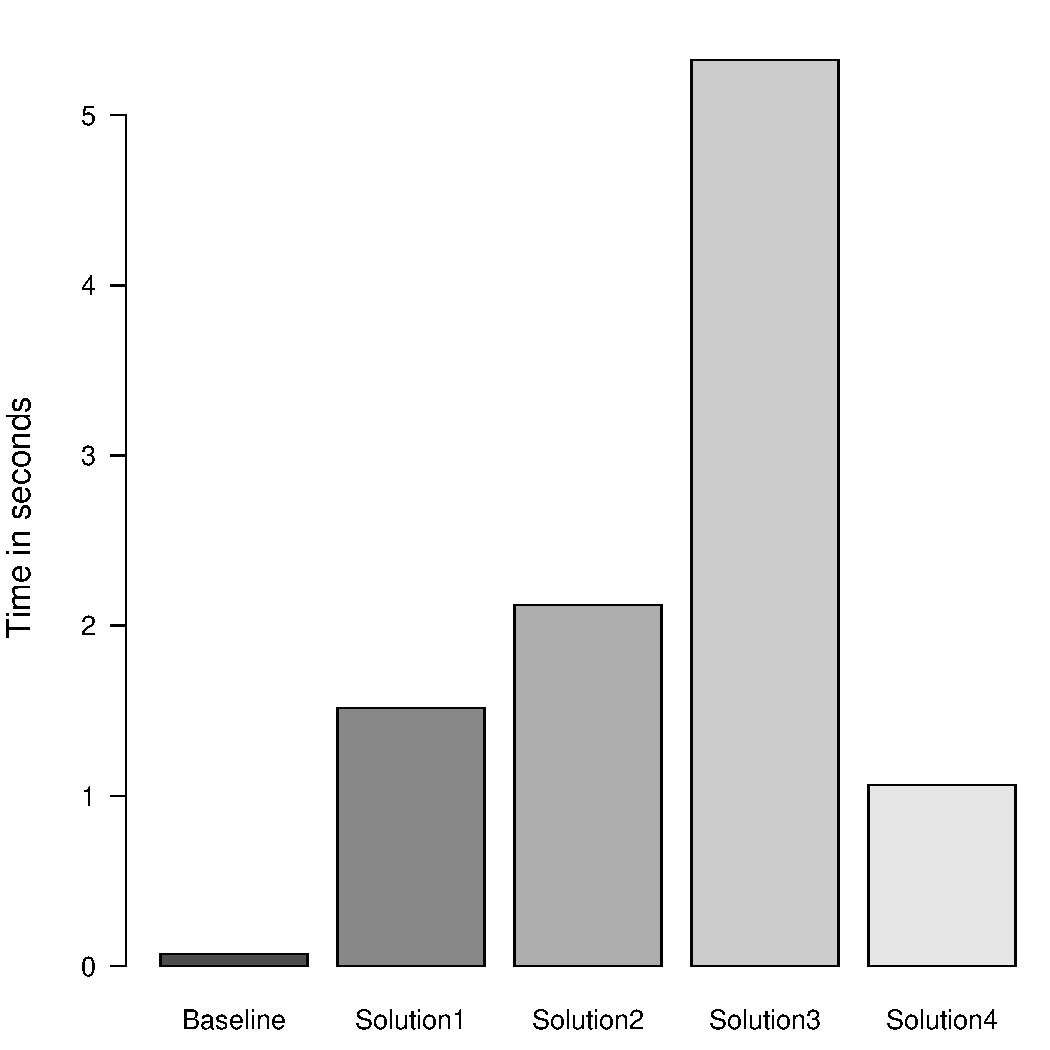
\includegraphics[width=\W]{figure/result/barplot-delete_student-rt.pdf}}			
			\subfigure[Throughput]
			{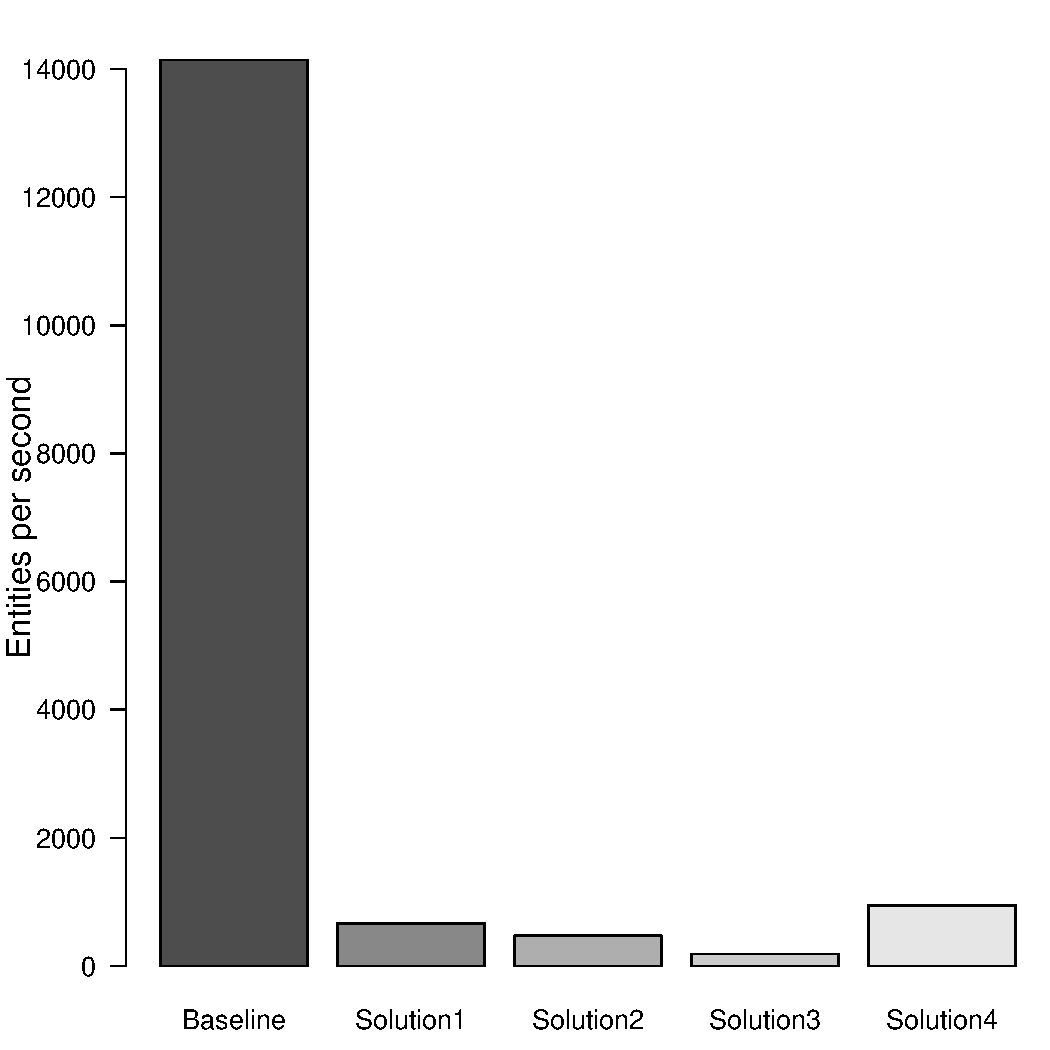
\includegraphics[width=\W]{figure/result/barplot-delete_student-tp.pdf}}
			\caption{Performance deleting students}\label{fres:delete-user}
% 		\end{figure} 
% \newpage	  
% 	\subsection{Course}
% 		\begin{figure}[H]
			\subfigure[Response time]
			{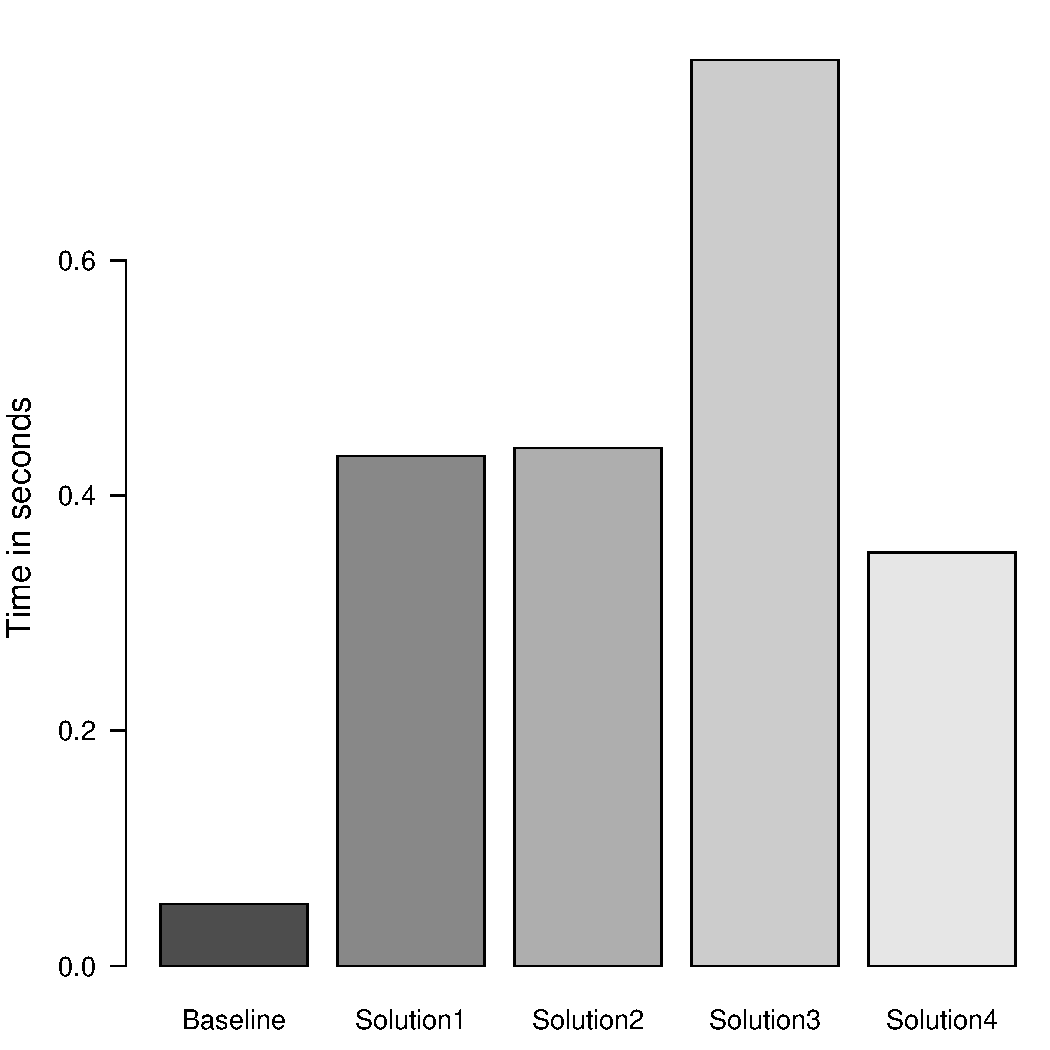
\includegraphics[width=\W]{figure/result/barplot-delete_course-rt.pdf}}
			\subfigure[Throughput]
			{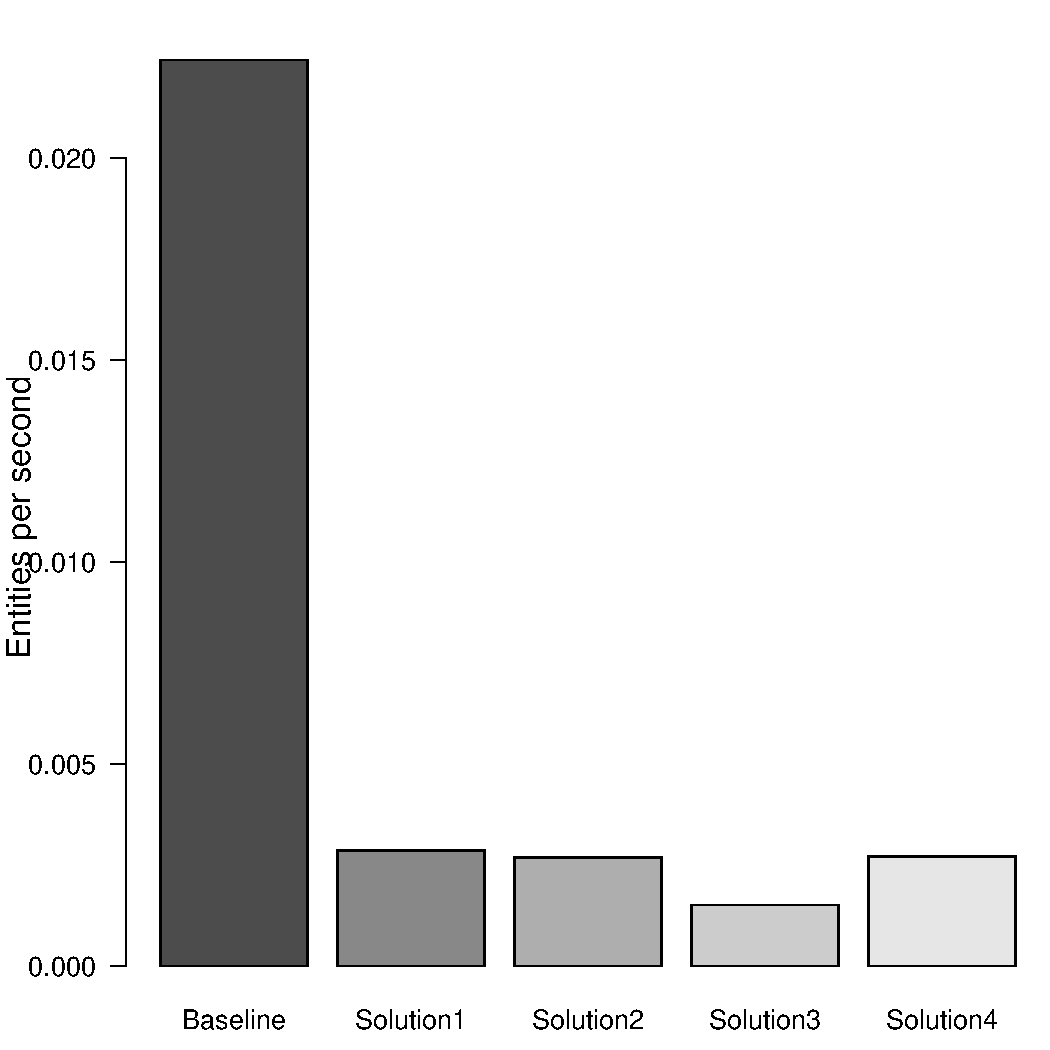
\includegraphics[width=\W]{figure/result/barplot-delete_course-tp.pdf}}
			\caption{Performance deleting courses}\label{fres:delete-course}
% 		\end{figure}	
% \newpage	 
% 	\subsection{Enrolment}
% 		\begin{figure}[H]
			\subfigure[Response time]
			{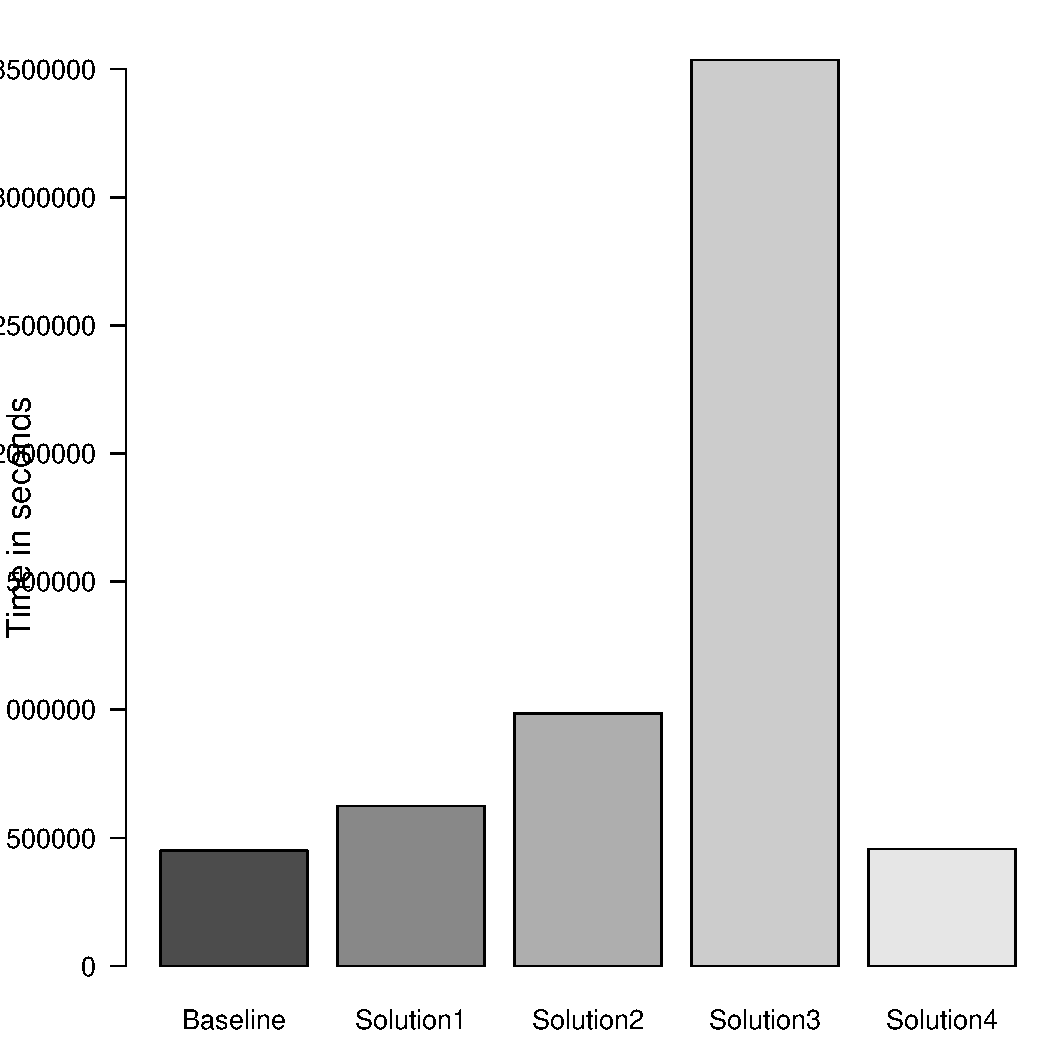
\includegraphics[width=\W]{figure/result/barplot-delete_enrolment-rt.pdf}}
			\subfigure[Throughput]
			{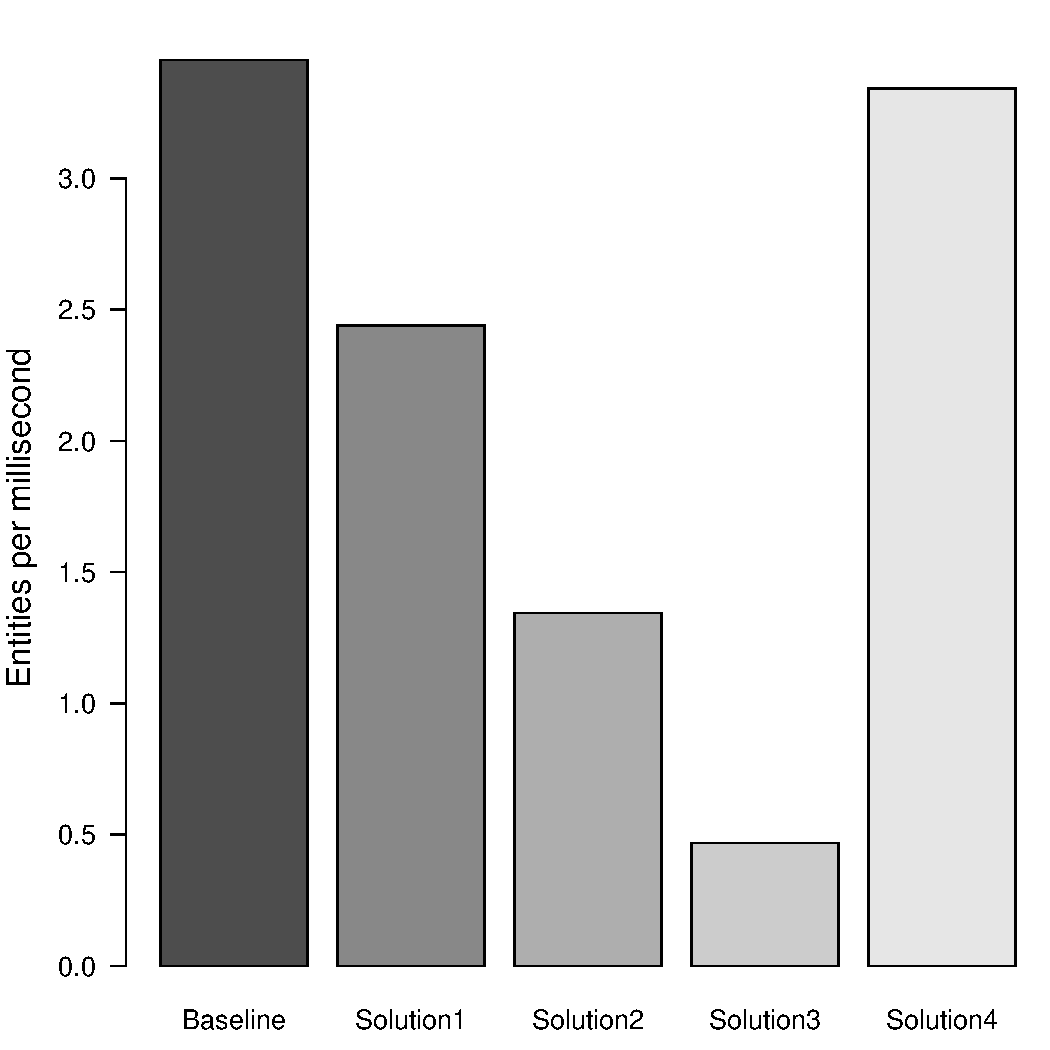
\includegraphics[width=\W]{figure/result/barplot-delete_enrolment-tp.pdf}}
			\caption{Performance deleting enrolments}\label{fres:delete-enrolment}
		\end{figure}
		
